\documentclass[a4paper]{report}

% Polish letters packages (for OS X)
\usepackage[utf8]{inputenc}
\usepackage{polski}
\usepackage[polish]{babel}

\usepackage{ragged2e}

\usepackage[T1]{fontenc}
\usepackage{textcomp}
\usepackage{lmodern}
\usepackage[a4paper, margin=1in]{geometry}
% do robienia tabel które mieszczą się na stronie (łamanie linii w kolumnach tabeli)
\usepackage{tabulary}
% do wrzucania obrazów
\usepackage{graphicx}
\usepackage{float}
% scieżka do folderu z plikami graficznymi
\graphicspath{{./images/}}
% do opisu tabel i rysunków
\usepackage{caption}
\captionsetup[table]{name=Tabela}
% do tabel żeby robić kreski (toprule, bottomrule itp)
\usepackage{booktabs}
% do kolorowania wierszy w tabeli
\usepackage{color, colortbl}
\definecolor{Gray}{gray}{0.75}
% do tworzenia własnych styli formatowania komórek tabel
\usepackage{array}
\newcolumntype{X}[1]{>{\raggedright\let\newline\\\arraybackslash\hspace{0pt}}m{#1}}
% do schowania napisu rozdzial n
\usepackage{titlesec} 
\titleformat{\chapter}[display]{\normalfont\bfseries}{}{0pt}{\Huge}
% do dodawania listingów kodu
\usepackage{listings}
% obracanie strony do landsacape
\usepackage{pdflscape}

\title{\huge Układy Cyfrowe i Systemy Wbudowane 2\\Projekt Synthesia}
\date{} % pusta data
\author{Jan Luch\hspace{42pt} 218150  \\Dawid Aksamski\hspace{5pt} 218429}


\begin{document}

\frenchspacing
\pagenumbering{gobble}
\maketitle
\newpage

\tableofcontents
\newpage

\pagenumbering{arabic}

\chapter{Wstęp}
	\section{Cel i zakres}
	Celem projektu było zaimplementowanie gry $"$Synthesia$"$, pozwalającej na naukę gry na pianinie poprzez naciskanie odpowiednich klawiszy w zależności od wyświetlającej się na ekranie animacji, dzięki czemu odtwarzany był odpowiedni dźwięk gamy.\\
	
Początkowo zakres projektu obejmował:
	\begin{enumerate}
	\item Wyświetlanie animacji zapisanej w pamięci układu melodii
	\item Kontrolowanie przebiegu gry poprzez odtwarzanie dźwięku, jeśli naciśnięty został odpowiedni \\klawisz zgodny z animacją
	\item Kontrolowanie przebiegu gry poprzez zatrzymywanie animacji w przypadku naciśnięcia złego \\klawisza
	\end{enumerate}
	
W trakcie wykonywania projektu jego zakres się zmienił, przez co jego końcowa wersja obejmuje:
	\begin{enumerate}
	\item Wyświetlanie animacji zapisanej melodii
	\item Odgrywanie zapisanej  melodii, ściśle związanej z wyświetlaną animacją - pozytywka
	\item Możliwość zmiany trybu na grę swobodną, co powoduje wyłączenie odtwarzania zapisanej \\melodii oraz wstrzymanie animacji, jednocześnie umożliwiając wygrywanie melodii przy użyciu klawiatury
	\end{enumerate}
	
	Projekt z planowanej gry edukacyjnej został zmodyfikowany do pozytywki odtwarzającej zapisaną \\w pamięci układu melodią wraz z jej wizualizacją na ekranie oraz z możliwością tzw. $"$gry swobodnej$"$.
	\section{Sprzęt}
		\par Do stworzenia systemu zastosowano układ FPGA Spartan-3E, 
		monitor VGA, brzęczyk 1 kHz, \\klawiaturę komputerową. Wszystkie peryferia, które zostały wykorzystane w projekcie
		zostały \\bezpośrednio podłączane do płytki Spartan-3E.\\\\
		\par Monitor został podłączony przy użyciu złącza D-SUB, 
		klawiatura komputerowa przy pomocy złącza PS/2, natomiast brzęczyk został podłączony pod odpowiednie piny wyjścia DAC OUT. Aby ułatwić 
		podłączanie brzęczyka do wyjścia DAC OUT ustawiony został odpowiedni sygnał sterujący pozwalający na przesłanie informacji na wszystkie 4 dostępne w tym 
		złączu porty, dzięki czemu jeden z kabli od brzęczyka mógł być podłączony do dowolnego z wymienionych pinów: \textbf{A},
		\textbf{B}, \textbf{C} lub \textbf{D}. Natomiast drugi kabelek został podłączony do uziemienia(pin \textbf{GND}).

\chapter{Projekt}
	\section{Opis}
	W projekcie zaimplementowano szereg modułów, co umożliwiło zarówno równoległą pracę nad nimi, \\jak również zmniejszyło odpowiedzialność i zależności między nimi. 
	Podział ten zapewnił również \\większą
	niezawodność całego układu oraz łatwość w lokalizowaniu ewentualnych błędów i 
	usterek \\systemu.
	\section{Hierarchia}
		\begin{figure}[h!]
			\centering
			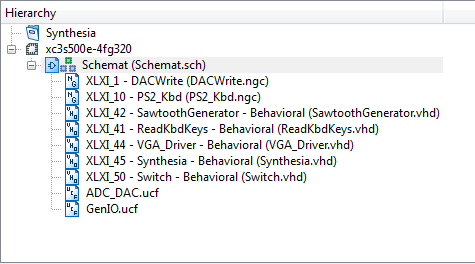
\includegraphics{hierarchy.png}
			\caption{Hierarchia plików źródłowych projektu}
		\end{figure}
				
		\begin{landscape}
			\subsection{Schemat}
				\begin{figure}[h!]
					\centering
					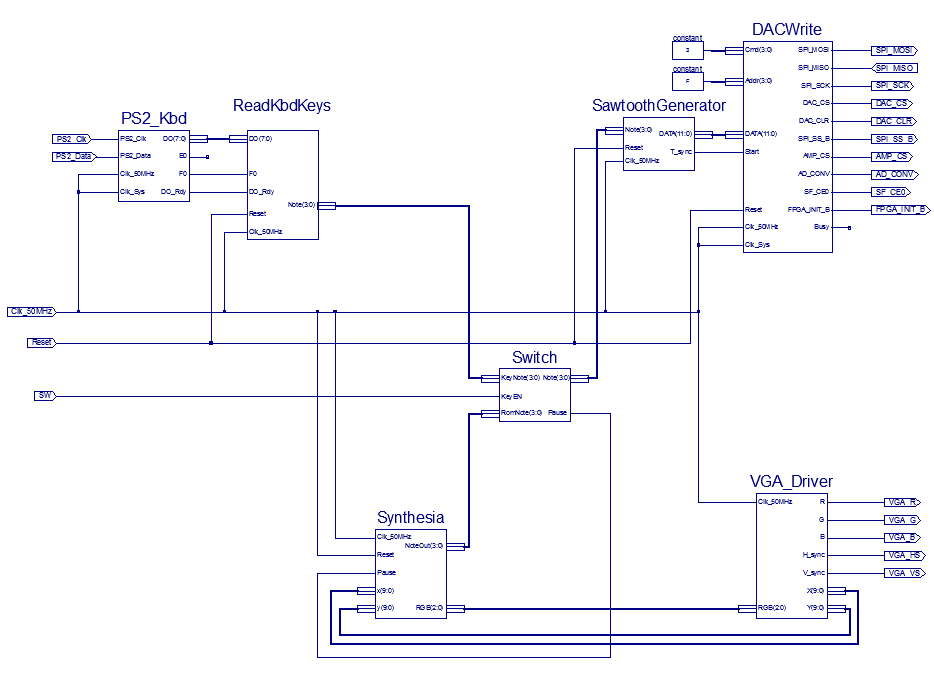
\includegraphics[width=1.1\textwidth]{schemat.png}
					\caption{Schemat systemu}
				\end{figure}
		\end{landscape}

\chapter{Moduły}
	\section{Generator Dźwięku}
		\subsection{Symbol}
			\begin{figure}[h!]
				\centering
				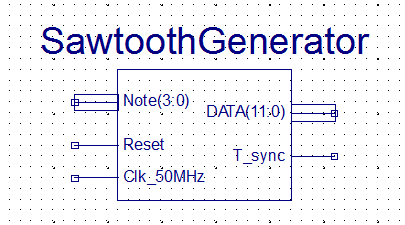
\includegraphics{sawtoothgenerator2.png}
				\caption{Moduł generujący falę piłokształtną}
			\end{figure}
			\vspace{15pt}
		\subsection{Porty}
		{\Large Wejścia:}
			\begin{itemize}	 
				\item \textbf{Note} - wektor w zakresie od 0 do 13 odpowiadający za wysokość generowanego dźwięku
				\item \textbf{Reset} - resetowanie procesu generowania fali piłokształtnej
				\item \textbf{Clk\_50MHz} - sygnał zegarowy
			\end{itemize}
		{\Large Wyjścia:}
			\begin{itemize} 
				\item \textbf{DATA} - wektor w zakresie od 0 do 4032 przesylany do modułu DAC\_Write
				\item \textbf{T\_sync} - sygnał startu przesyłania
			\end{itemize}
			\newpage
		\subsection{Najważniejsze sygnały i procesy}
		{\Large Sygnały:}
			\begin{itemize}
				\item \textbf{counter} - licznik pojedynczego przebiegu fali (jeden $"$ząb$"$ piły)
				\item \textbf{tickCounter} - licznik dzielący częstotliwość wejściową
				\item \textbf{ts} - sygnał startu przesyłania
				\item \textbf{index} - numer elementu tablicy zawierającej granice licznika dla poszczególnych częstotliwości dźwięku
				\item \textbf{pitch} - tablica typu \textbf{notes} zawierająca granice licznika dla dźwięków od C4 do C5 dla systemu równomiernie temperowanego, A4 = 440Hz
			\end{itemize}
		{\Large Procesy:}
			\begin{itemize}
			\item Proces odpowiedzialny za licznik dzielący częstotliwość oraz za generowanie sygnału startu przesyłania\\
				\lstinputlisting[language=VHDL, firstline=83, lastline=97,frame=single,tabsize=2]{SawtoothGenerator.vhd}
			\item Proces odpowiedzialny za licznik pojedynczego przebiegu fali\\
				\lstinputlisting[language=VHDL, firstline=100, lastline=111,frame=single,tabsize=2]{SawtoothGenerator.vhd}
			\item Proces odpowiedzialny za zwrócenie wektora wyjściowego na najstarszych bitach, ze względu na moduł DAC\_Write, który odczytuje najstarsze bity\\
				\lstinputlisting[language=VHDL, firstline=117, lastline=117,frame=single,tabsize=2]{SawtoothGenerator.vhd}
			\end{itemize}
		
		\begin{landscape}
			\subsection{Symulacja}
				\begin{figure}[h!]
					\centering
					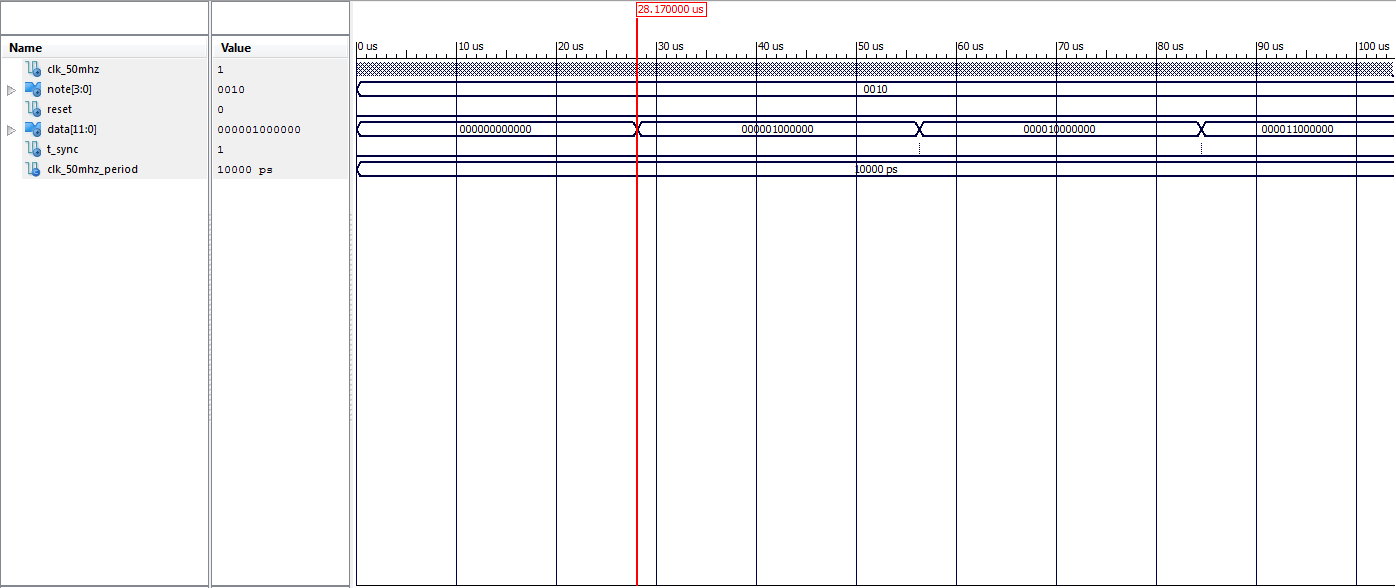
\includegraphics[width=1.6\textwidth]{sawtooth_generator_symulacja2.png}
					\caption{Symulacja modułu SawtoothGenerator}
				\end{figure}
\justify Symulacja pokazuje zmianę zmiennej DATA polegającą na inkrementacji 6 najstarszych bitów wektora. Po osiągnięciu wartości maksymalnej - 4032,\\ licznik jest zerowany. Wraz ze zmianą wartości wektora generowany jest impuls T\_sync.
		\end{landscape}
		
		\newpage
	\section{Sterownik VGA}
		\subsection{Symbol}
			\begin{figure}[h!]
				\centering
				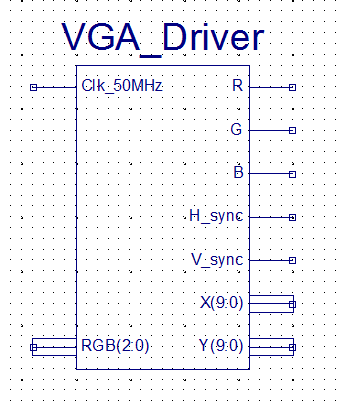
\includegraphics{vgadriver2.png}
				\caption{Moduł sterujący wyjściem VGA}
			\end{figure}
			
		\subsection{Porty}
			{\Large Wejścia:}
			\begin{itemize}	 
				\item \textbf{Clk\_50MHz} - sygnał zegarowy
				\item \textbf{RGB} - wektor w zakresie od 0 do 7 odpowiadający za kolor aktualnego piksela
			\end{itemize}
			{\Large Wyjścia:}
			\begin{itemize} 
				\item \textbf{R} - sygnał mówiący czy piksel ma mieć zapalony kolor czerwony
				\item \textbf{G} - sygnał mówiący czy piksel ma mieć zapalony kolor zielony
				\item \textbf{B} - sygnał mówiący czy piksel ma mieć zapalony kolor niebieski
				\item \textbf{H\_sync} - sygnał synchronizacji poziomej
				\item \textbf{V\_sync} - sygnał synchronizacji pionowej
				\item \textbf{X} - wektor z zakresu od 0 do 800, podaje on pozycję x w jakiej znajduje się naświetlany piksel
				\item \textbf{Y} - wektor z zakresu od 0 do 600, podaje on pozycję y w jakiej znajduje się naświetlany piksel
			\end{itemize}
			
		\subsection{Najważniejsze sygnały i procesy}
			{\Large Sygnały i stałe:}
			\begin{itemize}
				\item \textbf{hpixels} - stała przechowująca liczbę pikseli w poziomie wraz z marginesami
				\item \textbf{vlines} - stała przechowująca liczbę pikseli w pionie wraz z marginesami
				\item \textbf{maxWidth} - stała przechowująca liczbę pikseli ekranu w poziomie
				\item \textbf{maxHeight} - stała przechowująca liczbę pikseli ekranu w pionie
				\item \textbf{hbp} - stała przechowująca liczbę pikseli tylnego poziomego marginesu
				\item \textbf{hfp} - stała przechowująca liczbę pikseli przedniego poziomego marginesu
				\item \textbf{vbp} - stała przechowująca liczbę pikseli tylnego pionowego marginesu
				\item \textbf{vfp} - stała przechowująca liczbę pikseli przedniego pionowego marginesu
				\item \textbf{hpw} - stała przechowująca liczbę pikseli potrzebną do ustawienia działa elektronowego w poziomie
				\item \textbf{vpw} - stała przechowująca liczbę pikseli potrzebną do ustawienia działa elektronowego w pionie
				\item \textbf{hs} - sygnał synchronizacji poziomej
				\item \textbf{vs} - sygnał synchronizacji pionowej
				\item \textbf{screenEnabled} - zmienna boolowska mówiąca czy pozycja działa elektronowego znajduje się w obszarze ekranu
			\end{itemize}
			{\Large Procesy:}
			\begin{itemize}
				\item Proces odpowiedzialny za ustawianie sygnałów synchronizacji poziomej oraz pionowej gdy działo elektronowe
				znajduje się w polu ekranu \\
					\lstinputlisting[language=VHDL, firstline=73, lastline=101,frame=single,tabsize=2]{VGA_Driver.vhd}
				\item Proces odpowiedzialny za ustawienie sygnałów wyjściowych \textbf{X} i \textbf{Y}, mówiących o położeniu działa elektronowego
				w danym momencie. Ustawia on również zmienną boolowską \textbf{screenEnabled}, mówiącą o tym czy
				należy ustawić sygnał na portach \textbf{R}, \textbf{G} i \textbf{B}\\
					\lstinputlisting[language=VHDL, firstline=103, lastline=121,frame=single,tabsize=2]{VGA_Driver.vhd}
				\item Proces ustawiający na wyjściach \textbf{R}, \textbf{G} i \textbf{B} odpowiednie wartości z wektora wejściowego \textbf{RGB},
				gdy działo elektronowe znajduje się w obszarze ekranu lub \textbf{'0'} w przeciwnym wypadku.\\
					\lstinputlisting[language=VHDL, firstline=124, lastline=135,frame=single,tabsize=2]{VGA_Driver.vhd}
			\end{itemize}			
			
		\begin{landscape}
			\subsection{Symulacja}
				\begin{figure}[h!]
					\centering
					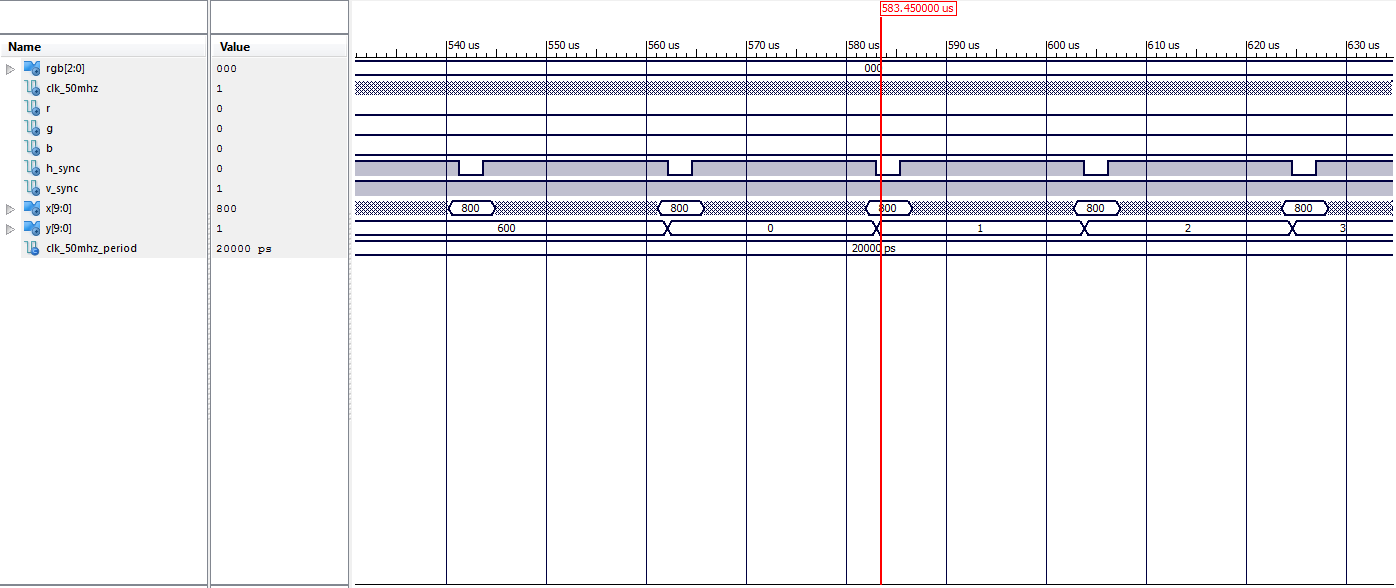
\includegraphics[width=1.6\textwidth]{vga_driver_symulacja2.png}
					\caption{Symulacja modułu VGA\_Driver}
				\end{figure}
			\justify
            Na symulacji można zauważyć jak szybko zmienia się wektor wyjściowy \textbf{X} oraz jak długo otrzymuje on wartość \textbf{800} co związane jest
            z czasem ustawienia się działa elektronowego w nowej linii. Ponadto widać na niej, że wartość sygnału wyjściowego \textbf{Y} zostaje
            zwiększona za każdym razem kiedy sygnał wyjściowy \textbf{X} osiąga swoją maksymalną wartość, czyli \textbf{800}. Tak samo dzieje się z
            sygnałem wyjściowym \textbf{Y} gdy osiągnie on swoją maksymalną wartość. Należy pamiętać, \\że po każdym osiągnięciu wartości maksymalnych
            przez sygnały wyjściowe \textbf{X} i \textbf{Y} następuje ustawienie się działa elektronowego co trwa ustaloną długość czasu.
		\end{landscape}
		
	\newpage
	\section{Przełącznik}
		\subsection{Symbol}	
			\begin{figure}[h!]
				\centering
				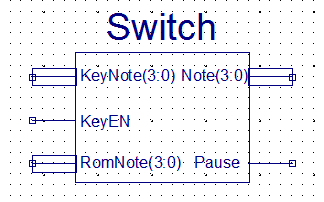
\includegraphics{switch2.png}
				\caption{Moduł sterujący trybem pracy systemu}
			\end{figure}
			
		\subsection{Porty}
			{\Large Wejścia:}
			\begin{itemize}	 
				\item \textbf{KeyNote} - wektor w zakresie od 0 do 13 odpowiadający numerowi przychodzącej nuty z modułu klawiatury
				\item \textbf{KeyEN} - ustawianie trybu w jakim ma działać urządzenie (\textbf{1} - klawiatura, \textbf{0} - pozytywka)
				\item \textbf{RomNote} - wektor w zakresie od 0 do 13 odpowiadający numerowi przychodzącej nuty z modułu pozytywki
			\end{itemize}
			{\Large Wyjścia:}
			\begin{itemize} 
				\item \textbf{Note} - wektor w zakresie od 0 do 13 ustawiany w zależności od trybu w jakim pracuje urządzenie
				\item \textbf{Pause} - sygnał zatrzymujący animację pozytywki
			\end{itemize}
			
		\subsection{Najważniejsze sygnały i procesy}
			{\Large Procesy:}
			\begin{itemize}
				\item Proces odpowiedzialny za ustawianie wektora wyjściowego \textbf{Note} w zależności od sygnału \textbf{KeyEN}\\
					\lstinputlisting[language=VHDL, firstline=43, lastline=43,frame=single,tabsize=2]{Switch.vhd}
				\item Proces odpowiedzialny za ustawianie sygnału pauzy w zależności od sygnału \textbf{KeyEN}\\
					\lstinputlisting[language=VHDL, firstline=44, lastline=44,frame=single,tabsize=2]{Switch.vhd}
			\end{itemize}
	
		\begin{landscape}
			\subsection{Symulacja}
				\begin{figure}[h!]
					\centering
					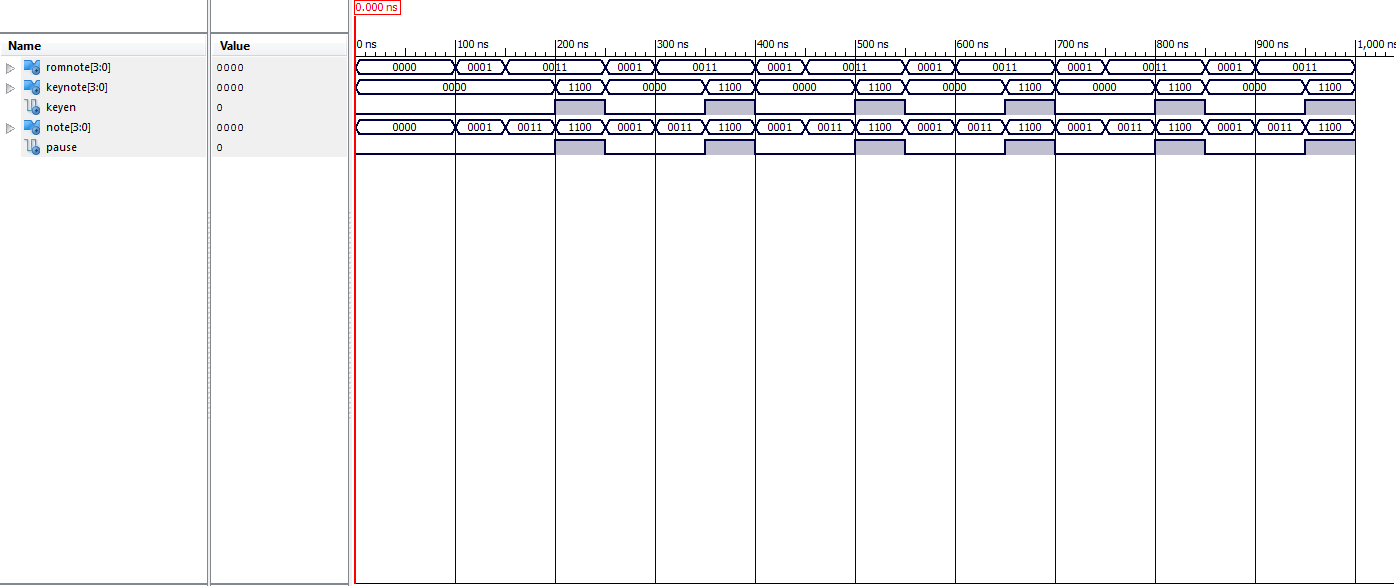
\includegraphics[width=1.6\textwidth]{switch_symulacja2.png}
					\caption{Symulacja modułu Switch}
				\end{figure}
			\justify
            Na symulacji widać jak w zależności od sygnału \textbf{KeyEN} podawany jest na wyjście odpowiedni rodzaj sygnału Note. 
            \textbf{RomNote} jeśli \textbf{KeyEN = '0'} lub \textbf{KeyNote} jeśli \textbf{KeyEN = '1'}.
            Ponadto, jeżeli sygnał \textbf{KeyEN = '1'}, to sygnał \textbf{Pause = '1}' w celu zatrzymania animacji pozytywki.
		\end{landscape}
		
	\section{Czytnik kodów z klawiatury}
		\subsection{Symbol}
			\begin{figure}[h!]
				\centering				
				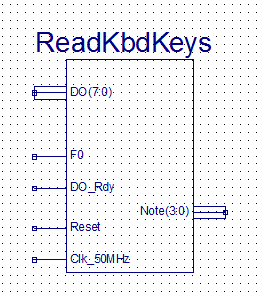
\includegraphics{readkbdkeys2.png}
				\caption{Moduł czytający kody skaningowe z klawiatury}
			\end{figure}
		\subsection{Porty}
			{\Large Wejścia:}
			\begin{itemize}	 
				\item \textbf{DO} - wektor w zakresie od 0 do 255 zawierający kod skaningowy wciśniętego klawisza
				\item \textbf{F0} - sygnał informujący o zwolnieniu klawisza
				\item \textbf{DO\_Rdy} - sygnał informujący o gotowości przesłaniu kodu wciśniętego klawisza
				\item \textbf{Reset} - sygnał resetu
				\item \textbf{Clk\_50MHz} - sygnał zegarowy
			\end{itemize}
			{\Large Wyjścia:}
			\begin{itemize} 
				\item \textbf{Note} - wektor w zakresie od 0 do 13 wysyłający numer klawisza, którego dźwięk ma zostać \\odtworzony
			\end{itemize}
		\subsection{Najważniejsze sygnały i procesy}
			{\Large Sygnały:}
			\begin{itemize}
				\item \textbf{input} - sygnał odpowiedzialny za zapamiętanie wektora sygnału wejściowego DO 
				w celu jego przechowywania, aż do momentu nadejścia sygnału zwolnienia klawisza
				\item \textbf{output} - sygnał wyjściowy przechowujący numer klawisza, którego dźwięk w danej chwili ma zostać odtworzony
			\end{itemize}
			\newpage
			{\Large Procesy:}
			\begin{itemize}
			\item Proces odpowiedzialny za ustawienie sygnału wyjściowego w zależności od wciśniętego w danej chwili klawisza klawiatury\\
				\lstinputlisting[language=VHDL, firstline=19, lastline=61,frame=single,tabsize=2]{ReadKbdKeys.vhd}
			\end{itemize}
			
		\begin{landscape}
			\subsection{Symulacja}
				\begin{figure}[h!]
					\centering
					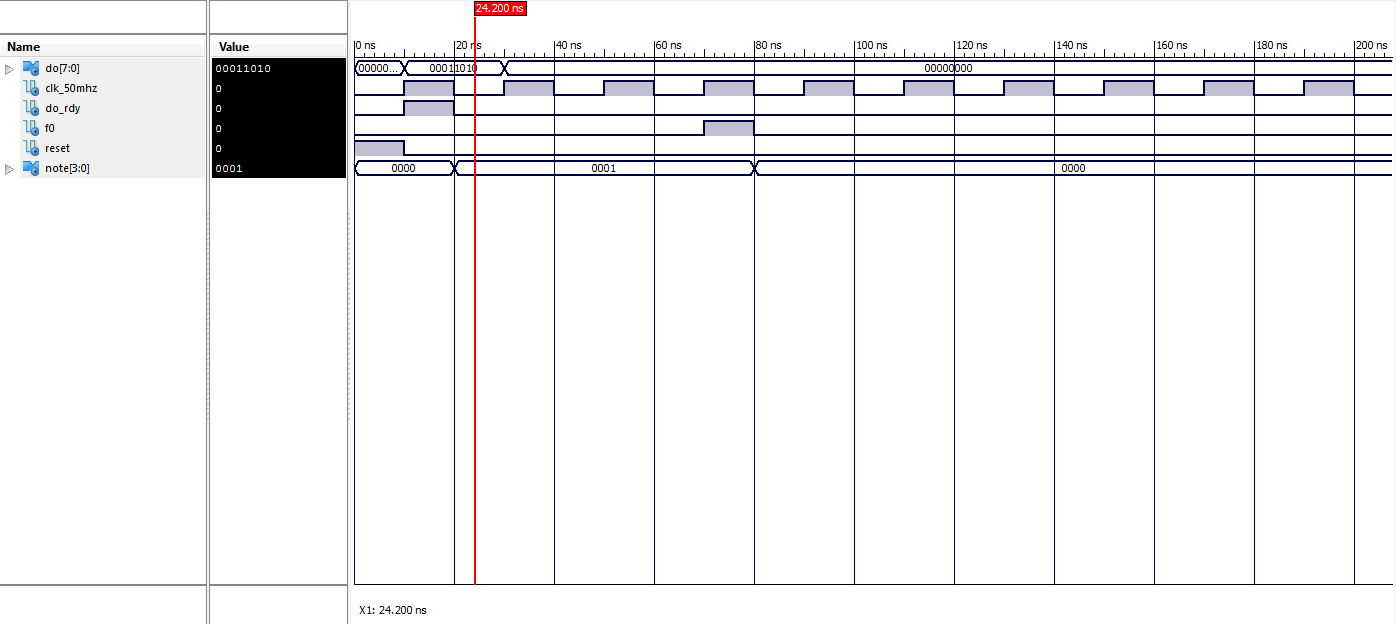
\includegraphics[width=1.6\textwidth]{readkbdkeys_symulacja2.png}
					\caption{Symulacja modułu ReadKbdKeys}
				\end{figure}
			\justify
            Symulacja pokazuje jak sygnał \textbf{Note} zostaje ustawiony na zadaną wartość po otrzymaniu przez moduł sygnału \textbf{DO\_Rdy}
            w zależności od tego jaki klawisz został wciśnięty(sygnał \textbf{DO} zawiera jego kod skaningowy). Chwilę później 
            sygnał \textbf{Note} zostaje ustawiony na \textbf{0}, po otrzymaniu przez moduł sygnału zwolnienia klawisza(sygnał \textbf{F0}).
		\end{landscape}
		
		\newpage
	\section{Synthesia}
		\subsection{Symbol}
			\begin{figure}[h!]
				\centering
				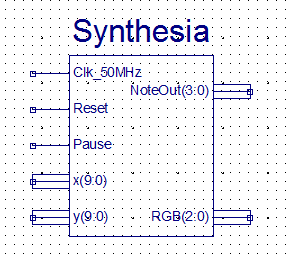
\includegraphics{synthesia2.png}
				\caption{Moduł zarządzający wyświetlaniem animacji oraz generowaniem melodii}
			\end{figure}
		\subsection{Porty}
		{\Large Wejścia:}
			\begin{itemize}	 
				\item	\textbf{Clk\_50MHz} - sygnał zegarowy
				\item \textbf{Reset} - resetowanie pracy modułu
				\item 	\textbf{Pause} - wstrzymywanie wyświetlania animacji
				\item \textbf{X, Y} - współrzędne aktualnie rysowanego punktu na ekranie
			\end{itemize}
		{\Large Wyjścia:}
			\begin{itemize} 
				\item 	\textbf{NoteOut} - wektor w zakresie od 0 do 13 odpowiadający za wysokość dźwięku do odtworzenia
				\item 	\textbf{RGB} - wektor w zakresie od 0 do 7 odpowiadający za wyświetlany kolor
			\end{itemize}
		\subsection{Najważniejsze sygnały i procesy}
		{\Large Sygnały:}
			\begin{itemize}
				\item \textbf{key\_position} - tablica elementów typu integer, przechowujących wartości pozycji horyzontalnej kolejnych dźwięków
				\item \textbf{should\_play} - sygnał typu STD\_LOGIC, przechowujący informację o tym, czy należy odtwarzać melodię z syntezatora
				\item \textbf{keys\_to\_display} - tablica elementów typu note - tablica 3 integerów - przechowujących kolejno: numer nuty, pozycję wertykalną graficznej reprezentacji dźwięku, wysokość graficznej reprezentacji dźwięku, jednocześnie odpowiadającą długości jego trwania
			\end{itemize}
			\newpage
		{\Large Procesy:}
			\begin{itemize}
			\item Proces odpowiedzialny za rysowanie graficznej reprezentacji dźwięków na ekranie\\
						\lstinputlisting[language=VHDL, firstline=134, lastline=181,frame=single,tabsize=2]{Synthesia.vhd}
						\newpage
			\item Proces odpowiedzialny za animowanie graficznej reprezentacji melodii\\
						\lstinputlisting[language=VHDL, firstline=183, lastline=196,frame=single,tabsize=2]{Synthesia.vhd}
			\item Proces odpowiedzialny za wybranie odpowiedniego dźwięku do odtworzenia na podstawie animacji\\
						\lstinputlisting[language=VHDL, firstline=198, lastline=259,frame=single,tabsize=2]{Synthesia.vhd}
			
			\end{itemize}
	\begin{landscape}
		\subsection{Symulacja}
		\begin{figure}[h!]
					\centering
					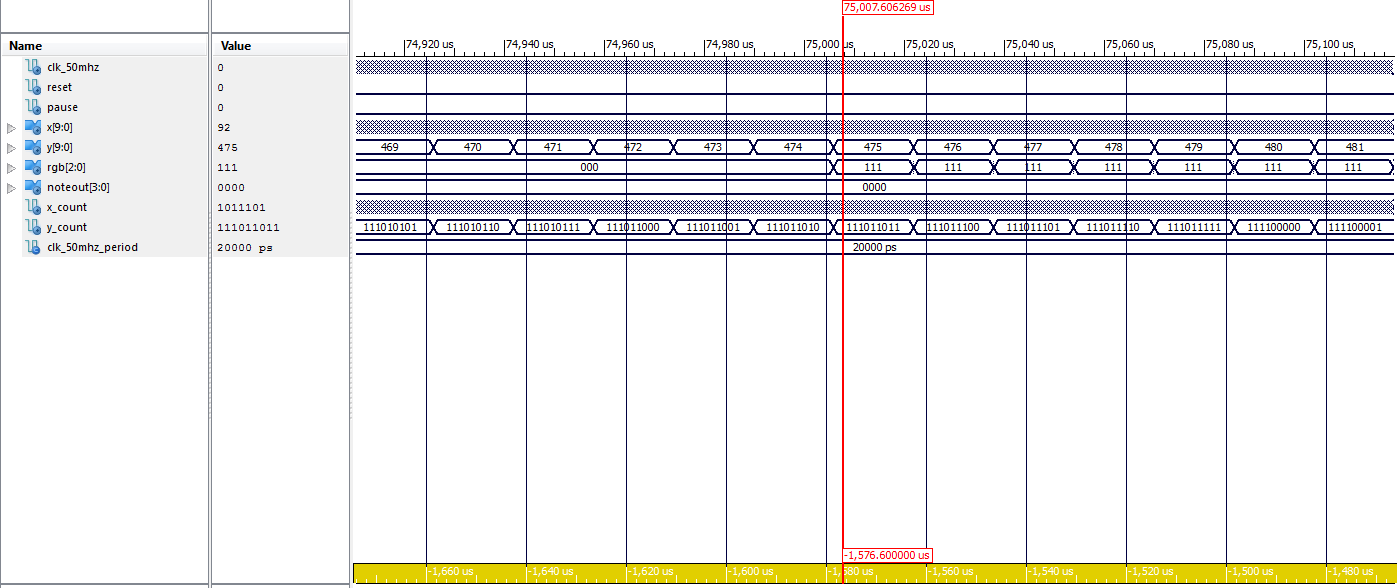
\includegraphics[width=1.6\textwidth]{synthesia_symulacja2.png}
					\caption{Symulacja modułu Synthesia}
				\end{figure}
\justify Symulacja pokazuje wyświetlenie dolnej "belki", która określa jaki dźwięk jest odgrywany. Belka ta wyświetlana jest dla wartości \textbf{Y} od 475 do 485, niezależnie od wartości zmiennej \textbf{X}.
		\end{landscape}
	
\chapter{Implementacja}
	Projekt został zaimplementowany w środowisku Xilinx ISE w wersji 14.7. Poprawność działania poszczególnych
	modułów całego projektu została przetestowana w środowisku ModelSim podczas pracy nad projektem jak i w jego fazie końcowej.
	Do poprawnej pracy układu niezbędna jest konfiguracja plików ADC\_DAC.ucf oraz GenIO.ucf, których listingi zostały przedstawione
	poniżej.\\
	
	ADC\_DAC.ucf \\
	\lstinputlisting[language=VHDL, firstline=1, lastline=23,frame=single,tabsize=2]{ADC_DAC.ucf}
	
	GenIO.ucf - zegar \\
	\lstinputlisting[language=VHDL, firstline=1, lastline=3,frame=single,tabsize=2]{GenIO.ucf}
	
	GenIO.ucf - przycisk reset \\
	\lstinputlisting[language=VHDL, firstline=12, lastline=17,frame=single,tabsize=2]{GenIO.ucf}
	
	GenIO.ucf - przełącznik trybu \\
	\lstinputlisting[language=VHDL, firstline=20, lastline=25,frame=single,tabsize=2]{GenIO.ucf}
	
	GenIO.ucf - port PS/2 \\
	\lstinputlisting[language=VHDL, firstline=47, lastline=50,frame=single,tabsize=2]{GenIO.ucf}
	
	GenIO.ucf - VGA \\
	\lstinputlisting[language=VHDL, firstline=53, lastline=59,frame=single,tabsize=2]{GenIO.ucf}

	\section{Rozmiar}
	
	Poniżej przedstawiono raporty wygenerowane przez środowisko Xilinx podczas implementacji.
	Wynika z niego, że projekt wymaga aż 6,188 LUT spośród 9312 dostępnych. Ponadto do implementacji
	zużyto 15\%  dostępnych przerzutników.
	
	\begin{figure}[h!]
				\centering
				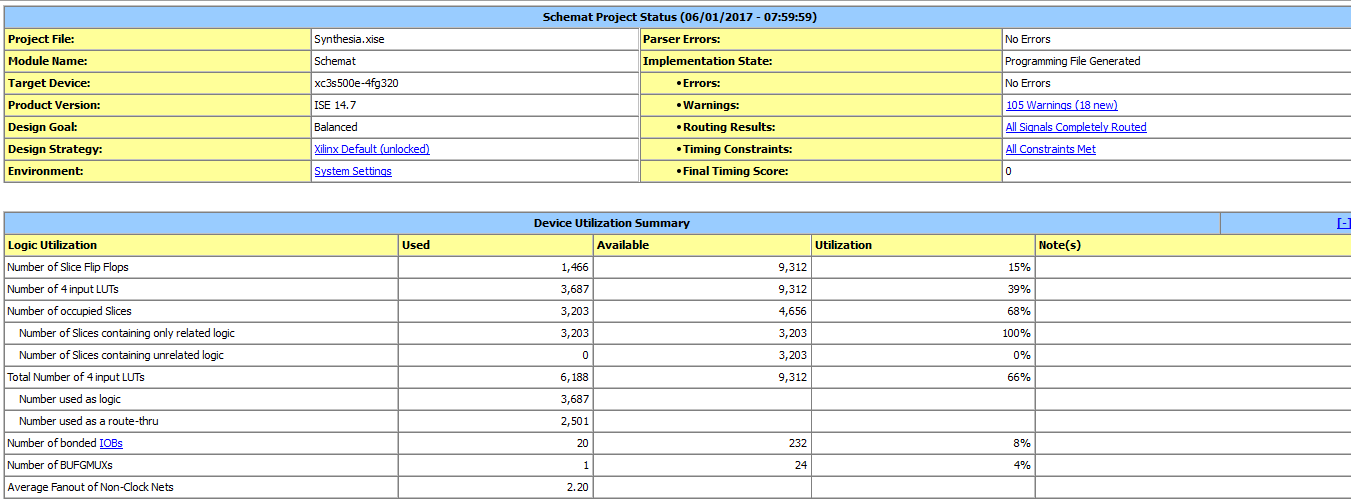
\includegraphics[width=1.0\textwidth]{report1.png}
				\caption{Raport cz. 1}
	\end{figure}	
	
	\newpage
	
	\begin{figure}[h!]
				\centering
				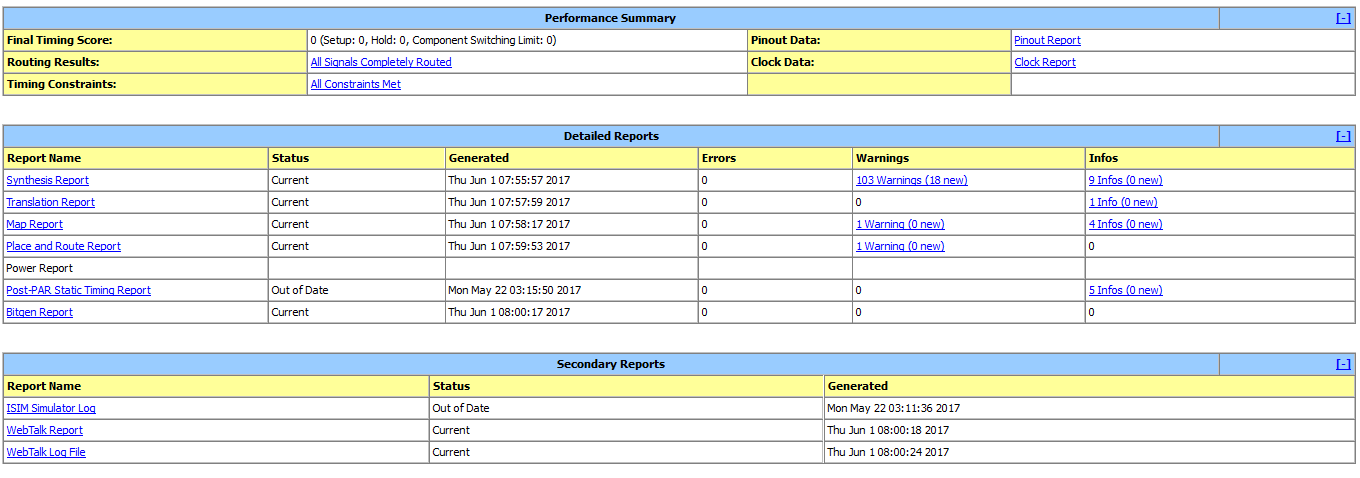
\includegraphics[width=1.0\textwidth]{report2.png}
				\caption{Raport cz. 2}
	\end{figure}	
	
	Częstotliwość maksymalna z jaką może pracować układ:
	\textbf{~20 GHz}
	 
	Maksymalne opóźnienie układu:
	\textbf{0.204000 ns}
	
	
		
	\section{Podręcznik użytkowania urządzenia}
	\par W celu użytkowania urządzenia należy wszystkie peryferia podłączyć do portów opisanych w sekcji sprzętu.
	
	\par Sterowanie trybem w jakim znajduje się urządzenie znajduje się pod przełącznikiem \textbf{SW3}. \\Stan wysoki
	oznacza tryb odtwarzania dźwięków z klawiatury, stan niski na przełączniku oznacza \\odtwarzanie melodii w formie
	pozytywki.
	\par Klawisze na klawiaturze komputerowej jakich użytkownik może używać w celu grania dźwięków to klawisze:
	\textbf{z}, \textbf{s}, \textbf{x}, \textbf{d}, \textbf{c}, \textbf{v}, \textbf{g}, \textbf{b}, \textbf{h}
	, \textbf{n}, \textbf{j}, \textbf{m} oraz \textbf{,}. Jest to cała oktawa klawiatury fortepianowej plus jeden
	klawisz z kolejnej oktawy(\textbf{,}).
	
	\par Do resetowania urządzenia służy przycisk \textbf{BTN South} znajdujący się na płytce Spartan-3E.
	
	Zdjęcia zestawu:\\
	
	
	\begin{figure}[h!]
				\centering
				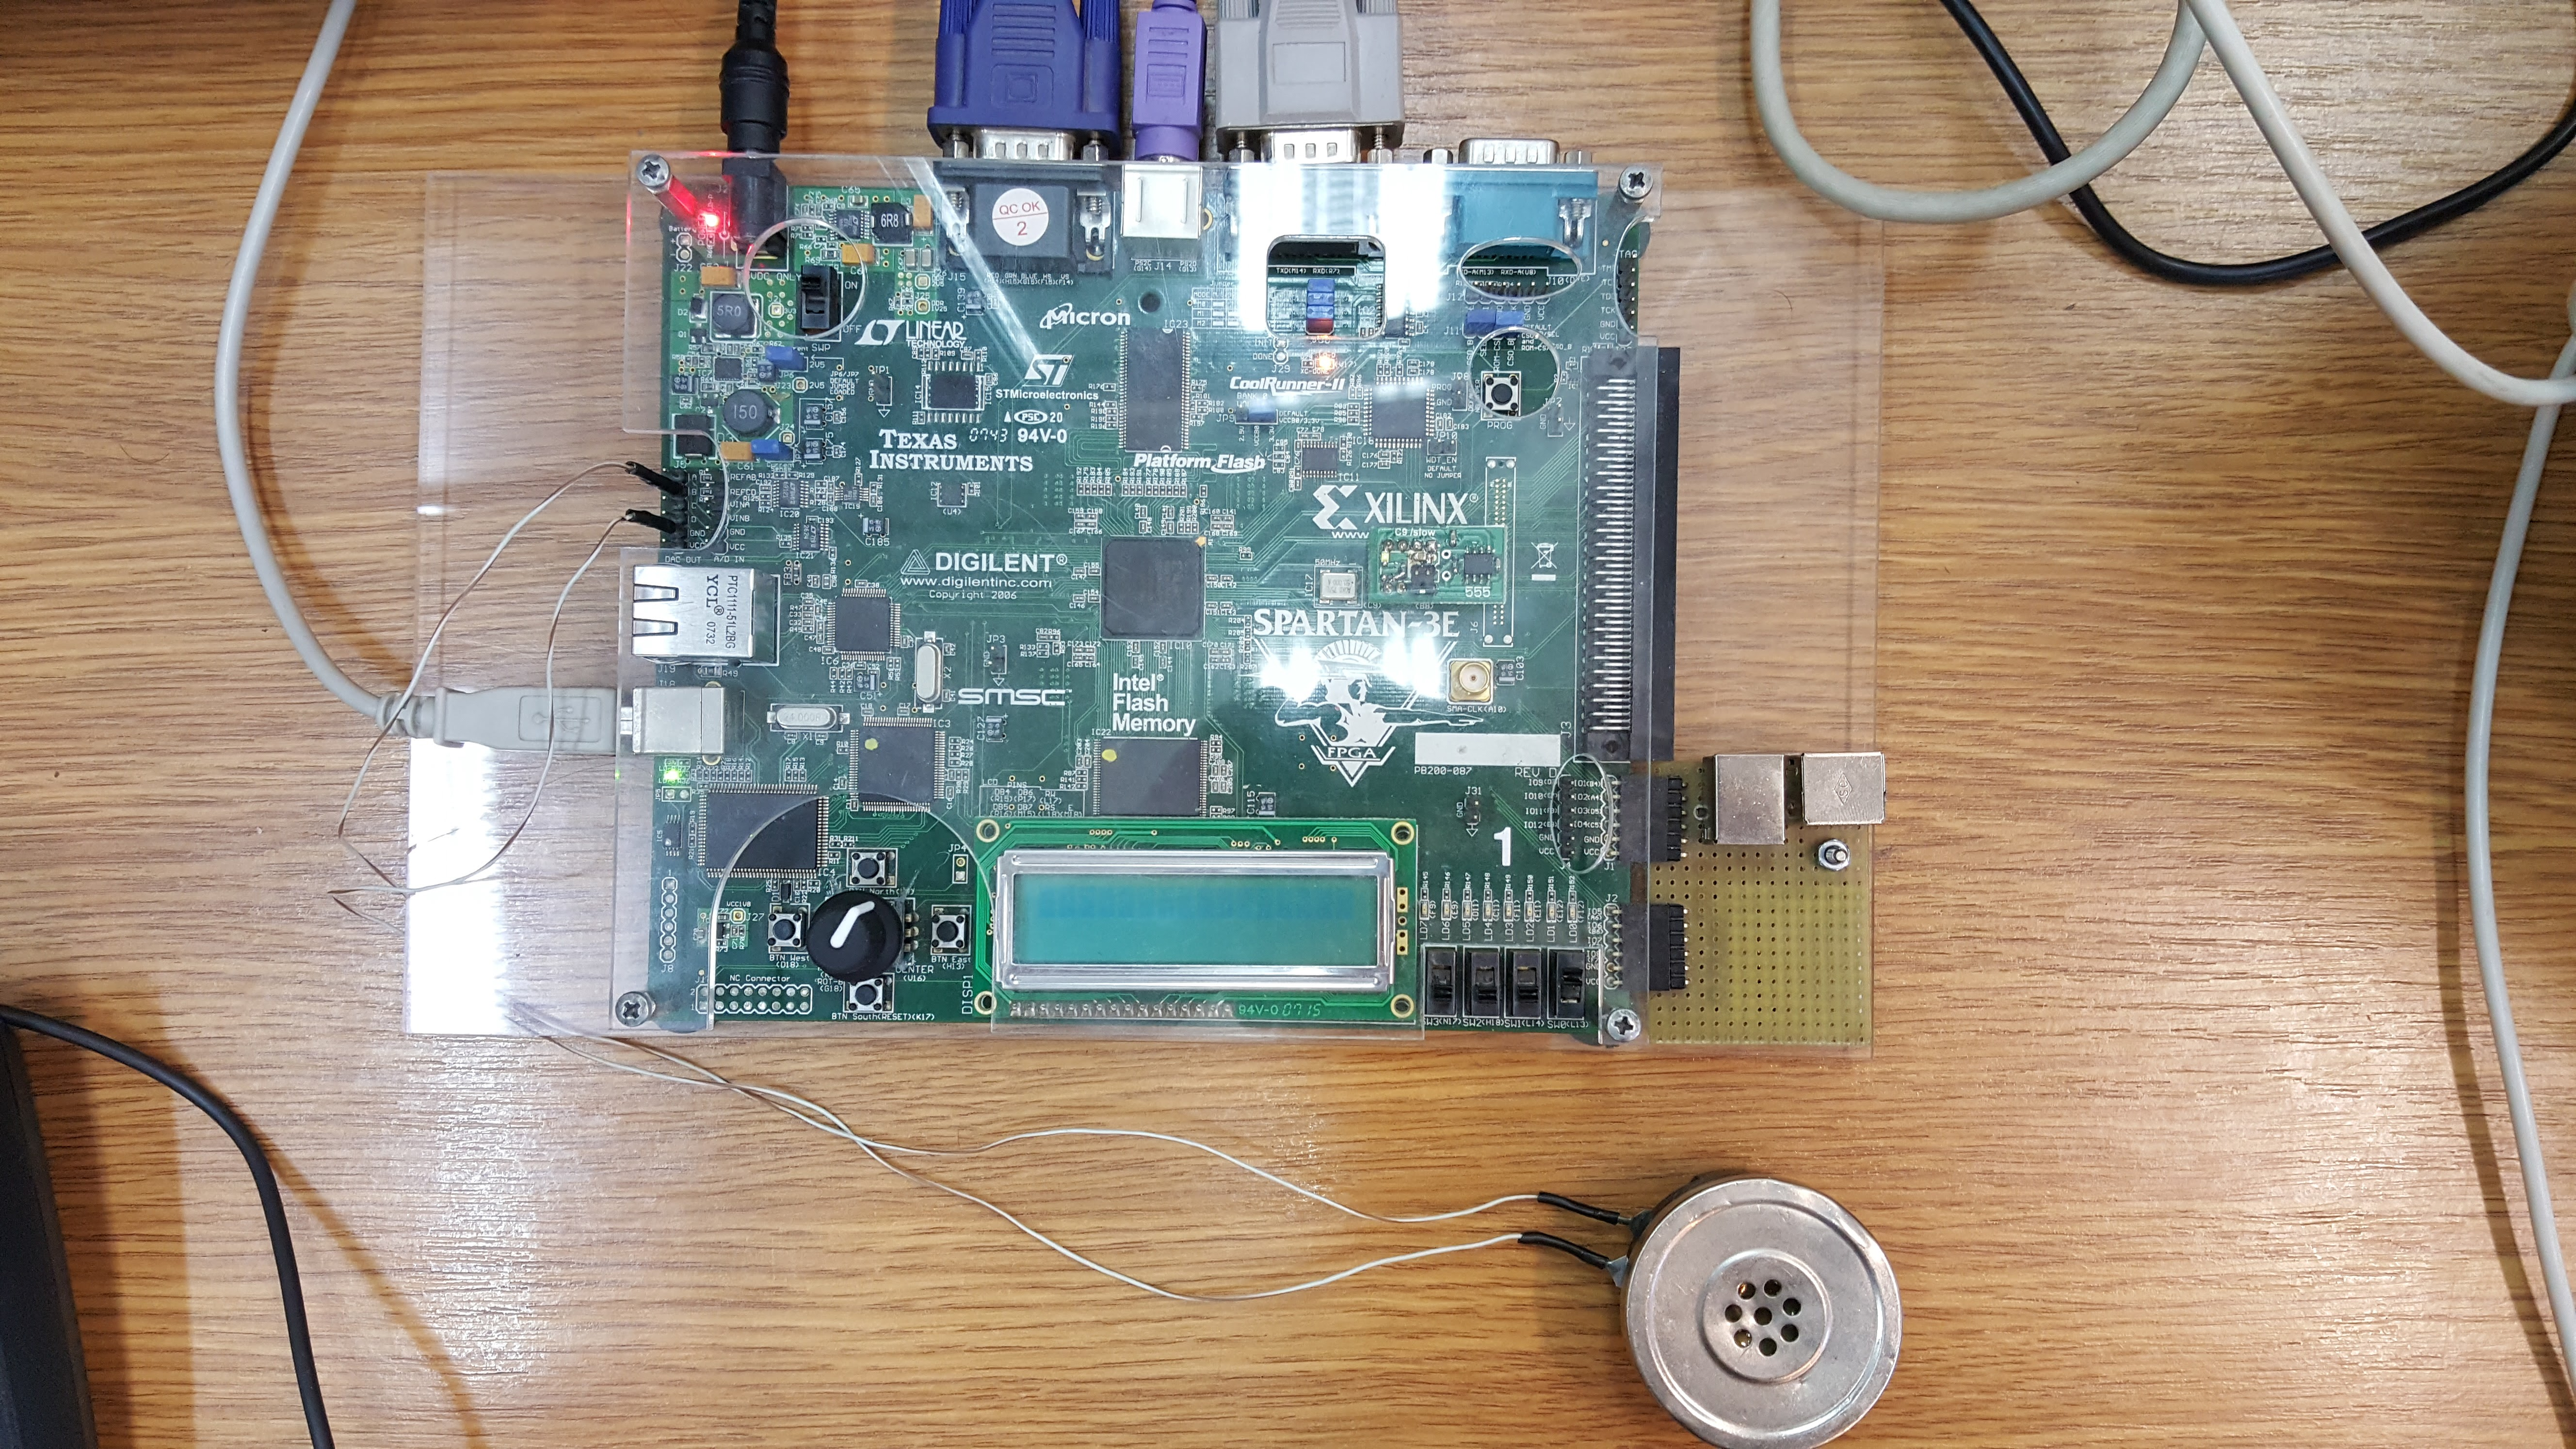
\includegraphics[width=1.0\textwidth]{zestaw_plytka_i_glosniczek2.jpg}
				\caption{Zestaw - płytka Spartan-3E i brzęczyk}
	\end{figure}	
	
	\begin{figure}[h!]
				\centering
				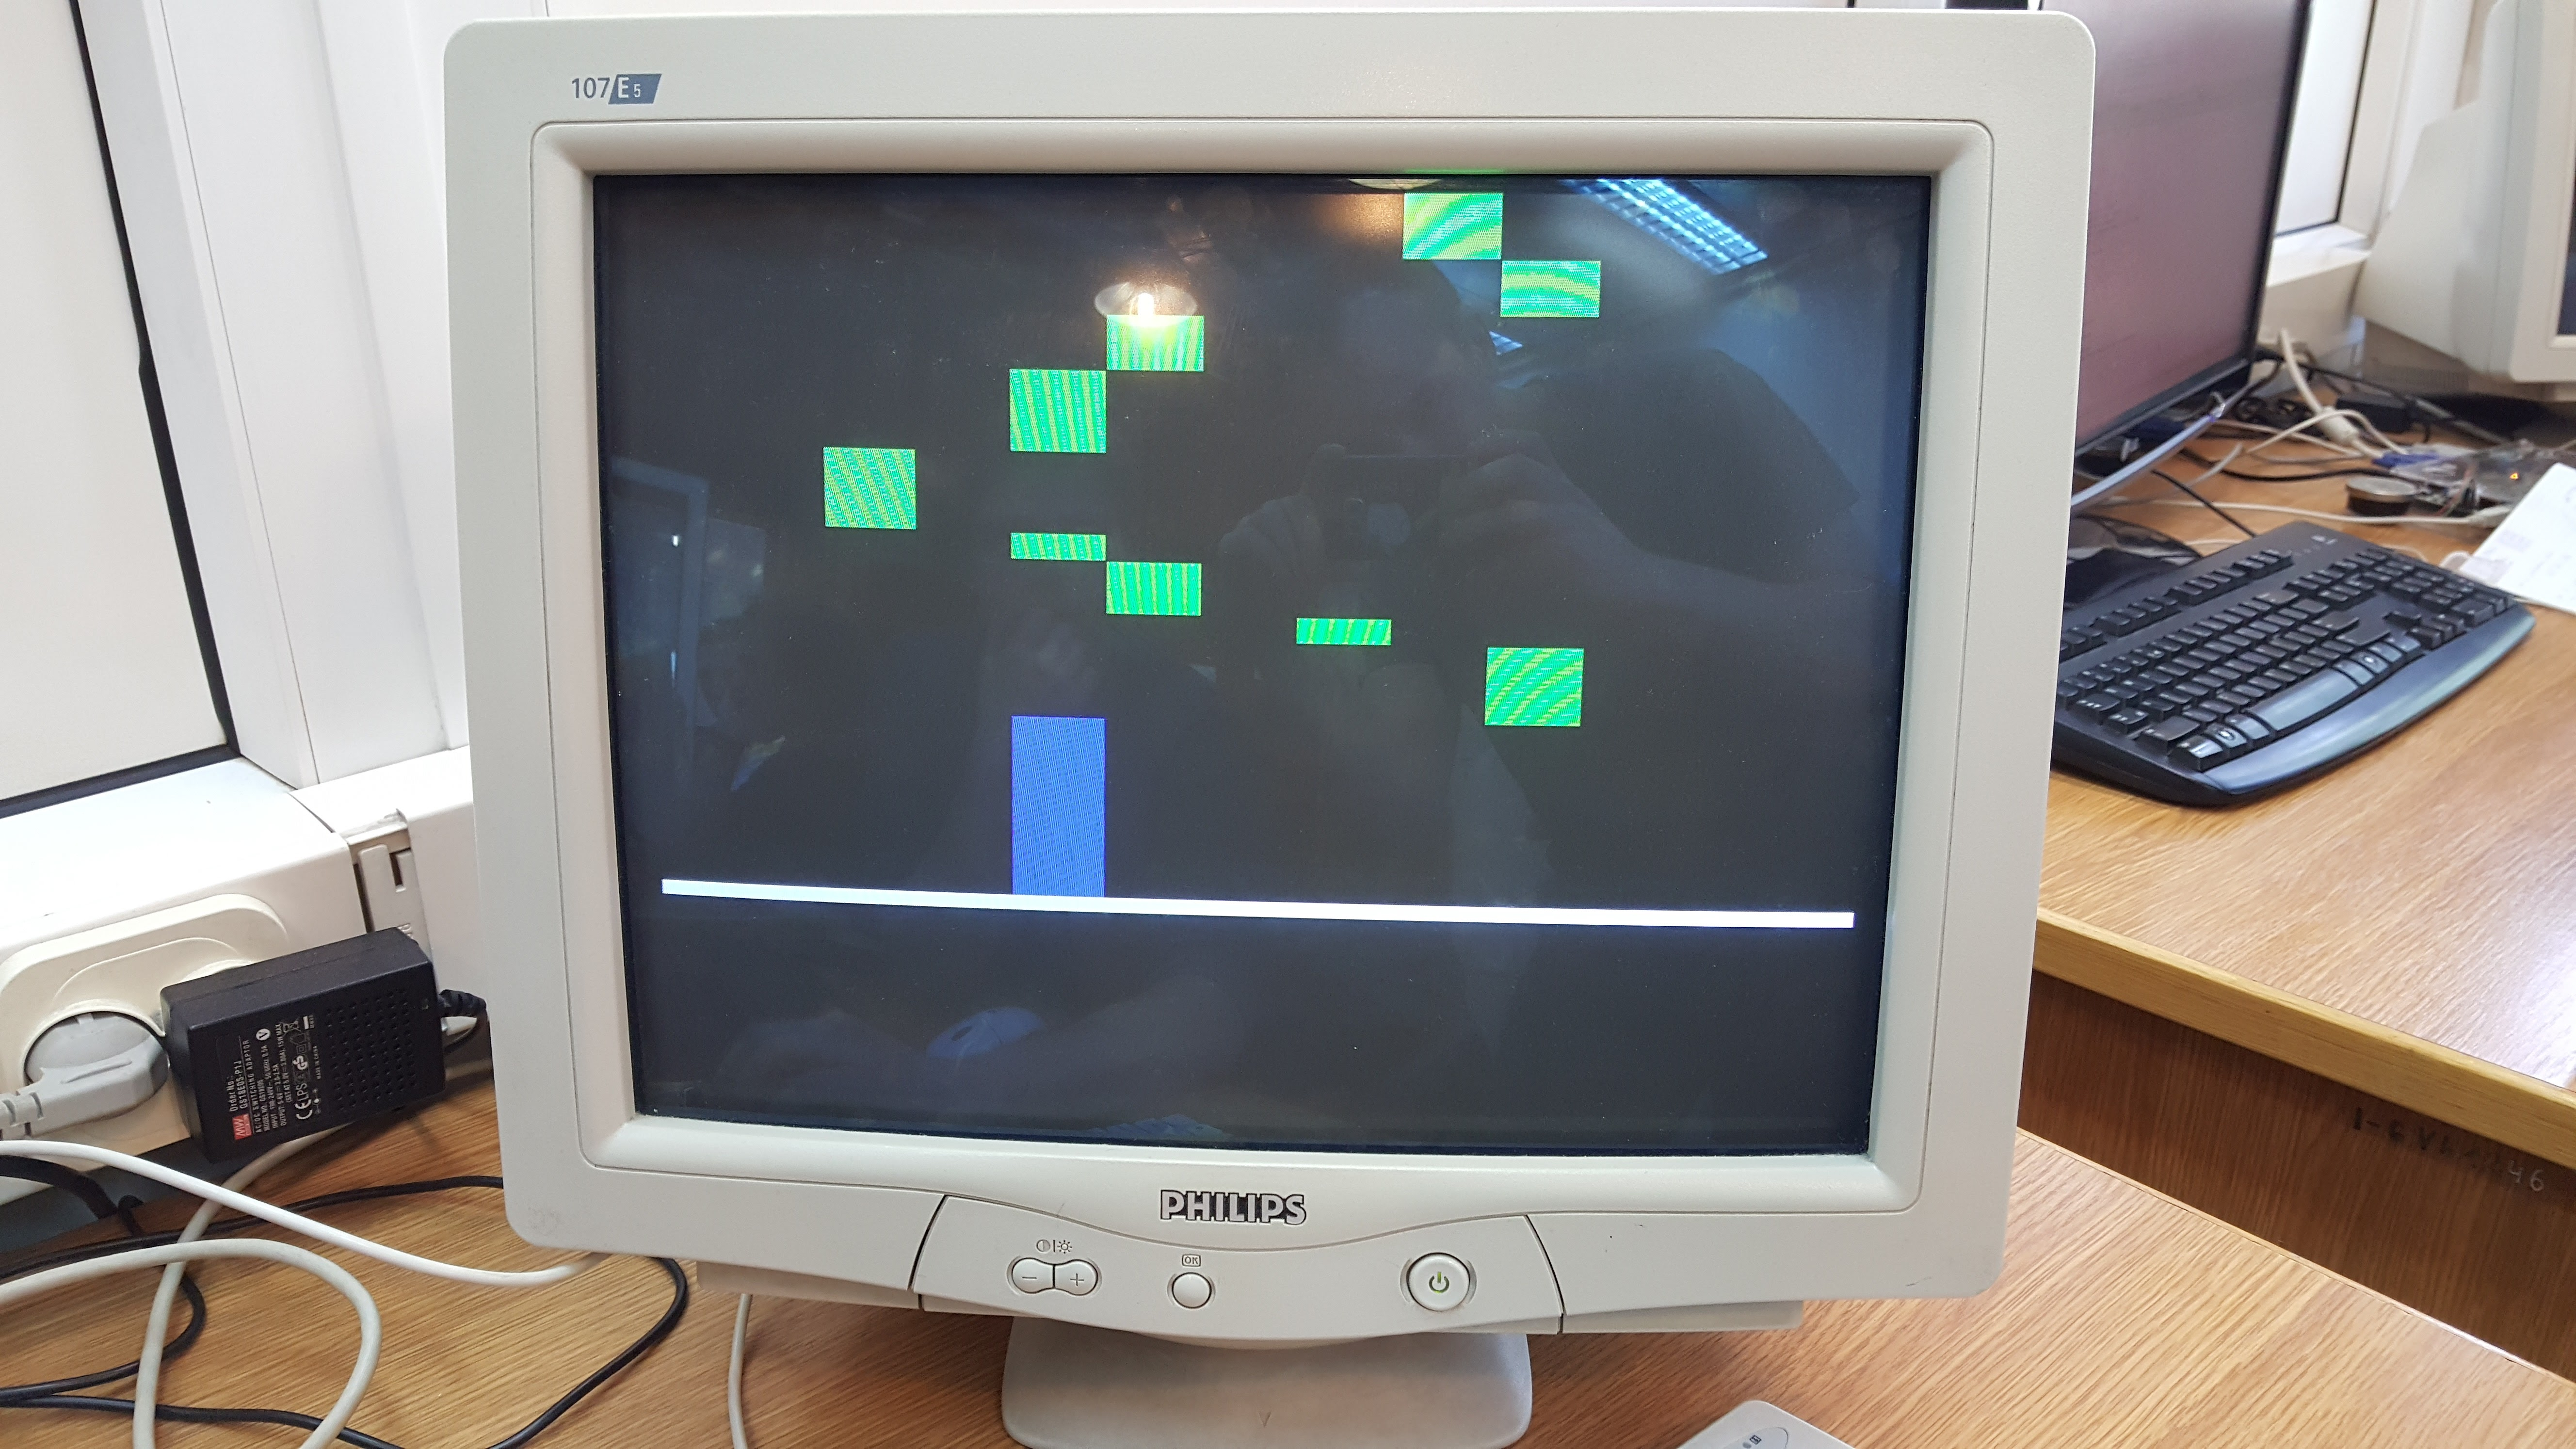
\includegraphics[width=1.0\textwidth]{zestaw_monitor3.jpg}
				\caption{Zestaw - monitor VGA}
	\end{figure}	
	
	\begin{figure}[h!]
				\centering
				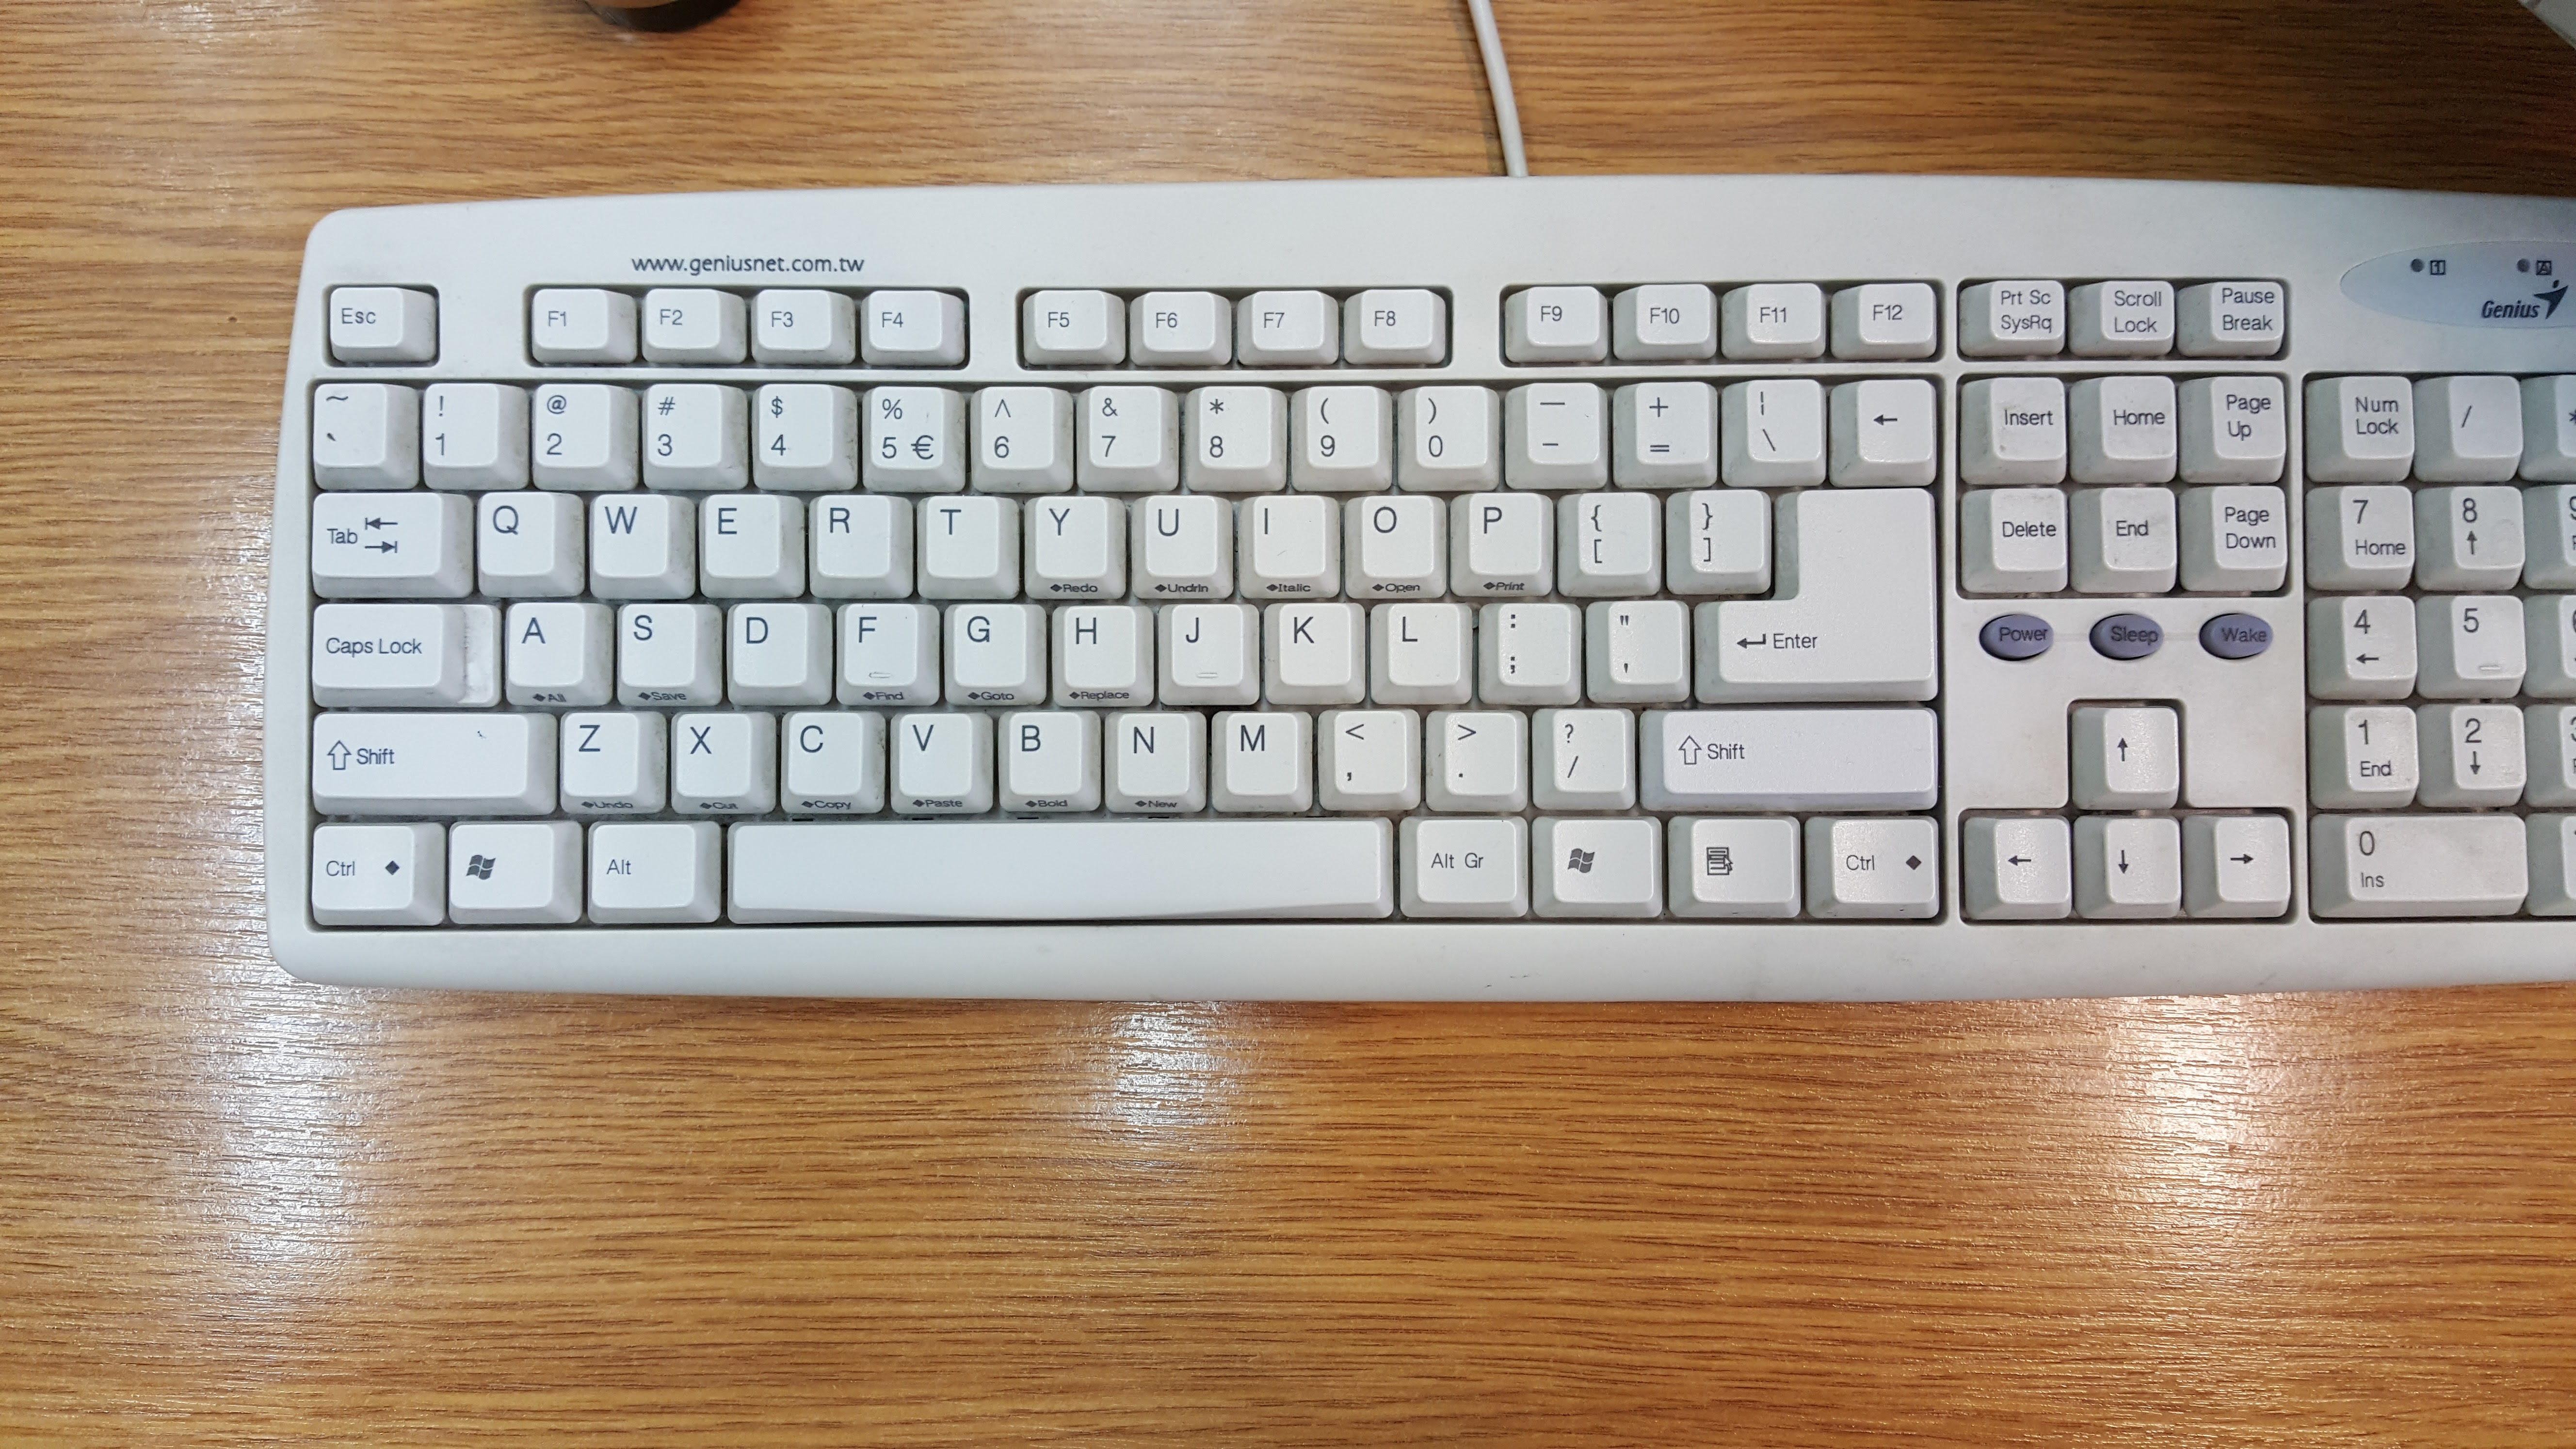
\includegraphics[width=1.0\textwidth]{zestaw_klawiatura.jpg}
				\caption{Zestaw - klawiatura komputerowa}
	\end{figure}	
	
		\begin{figure}[h!]
				\centering
				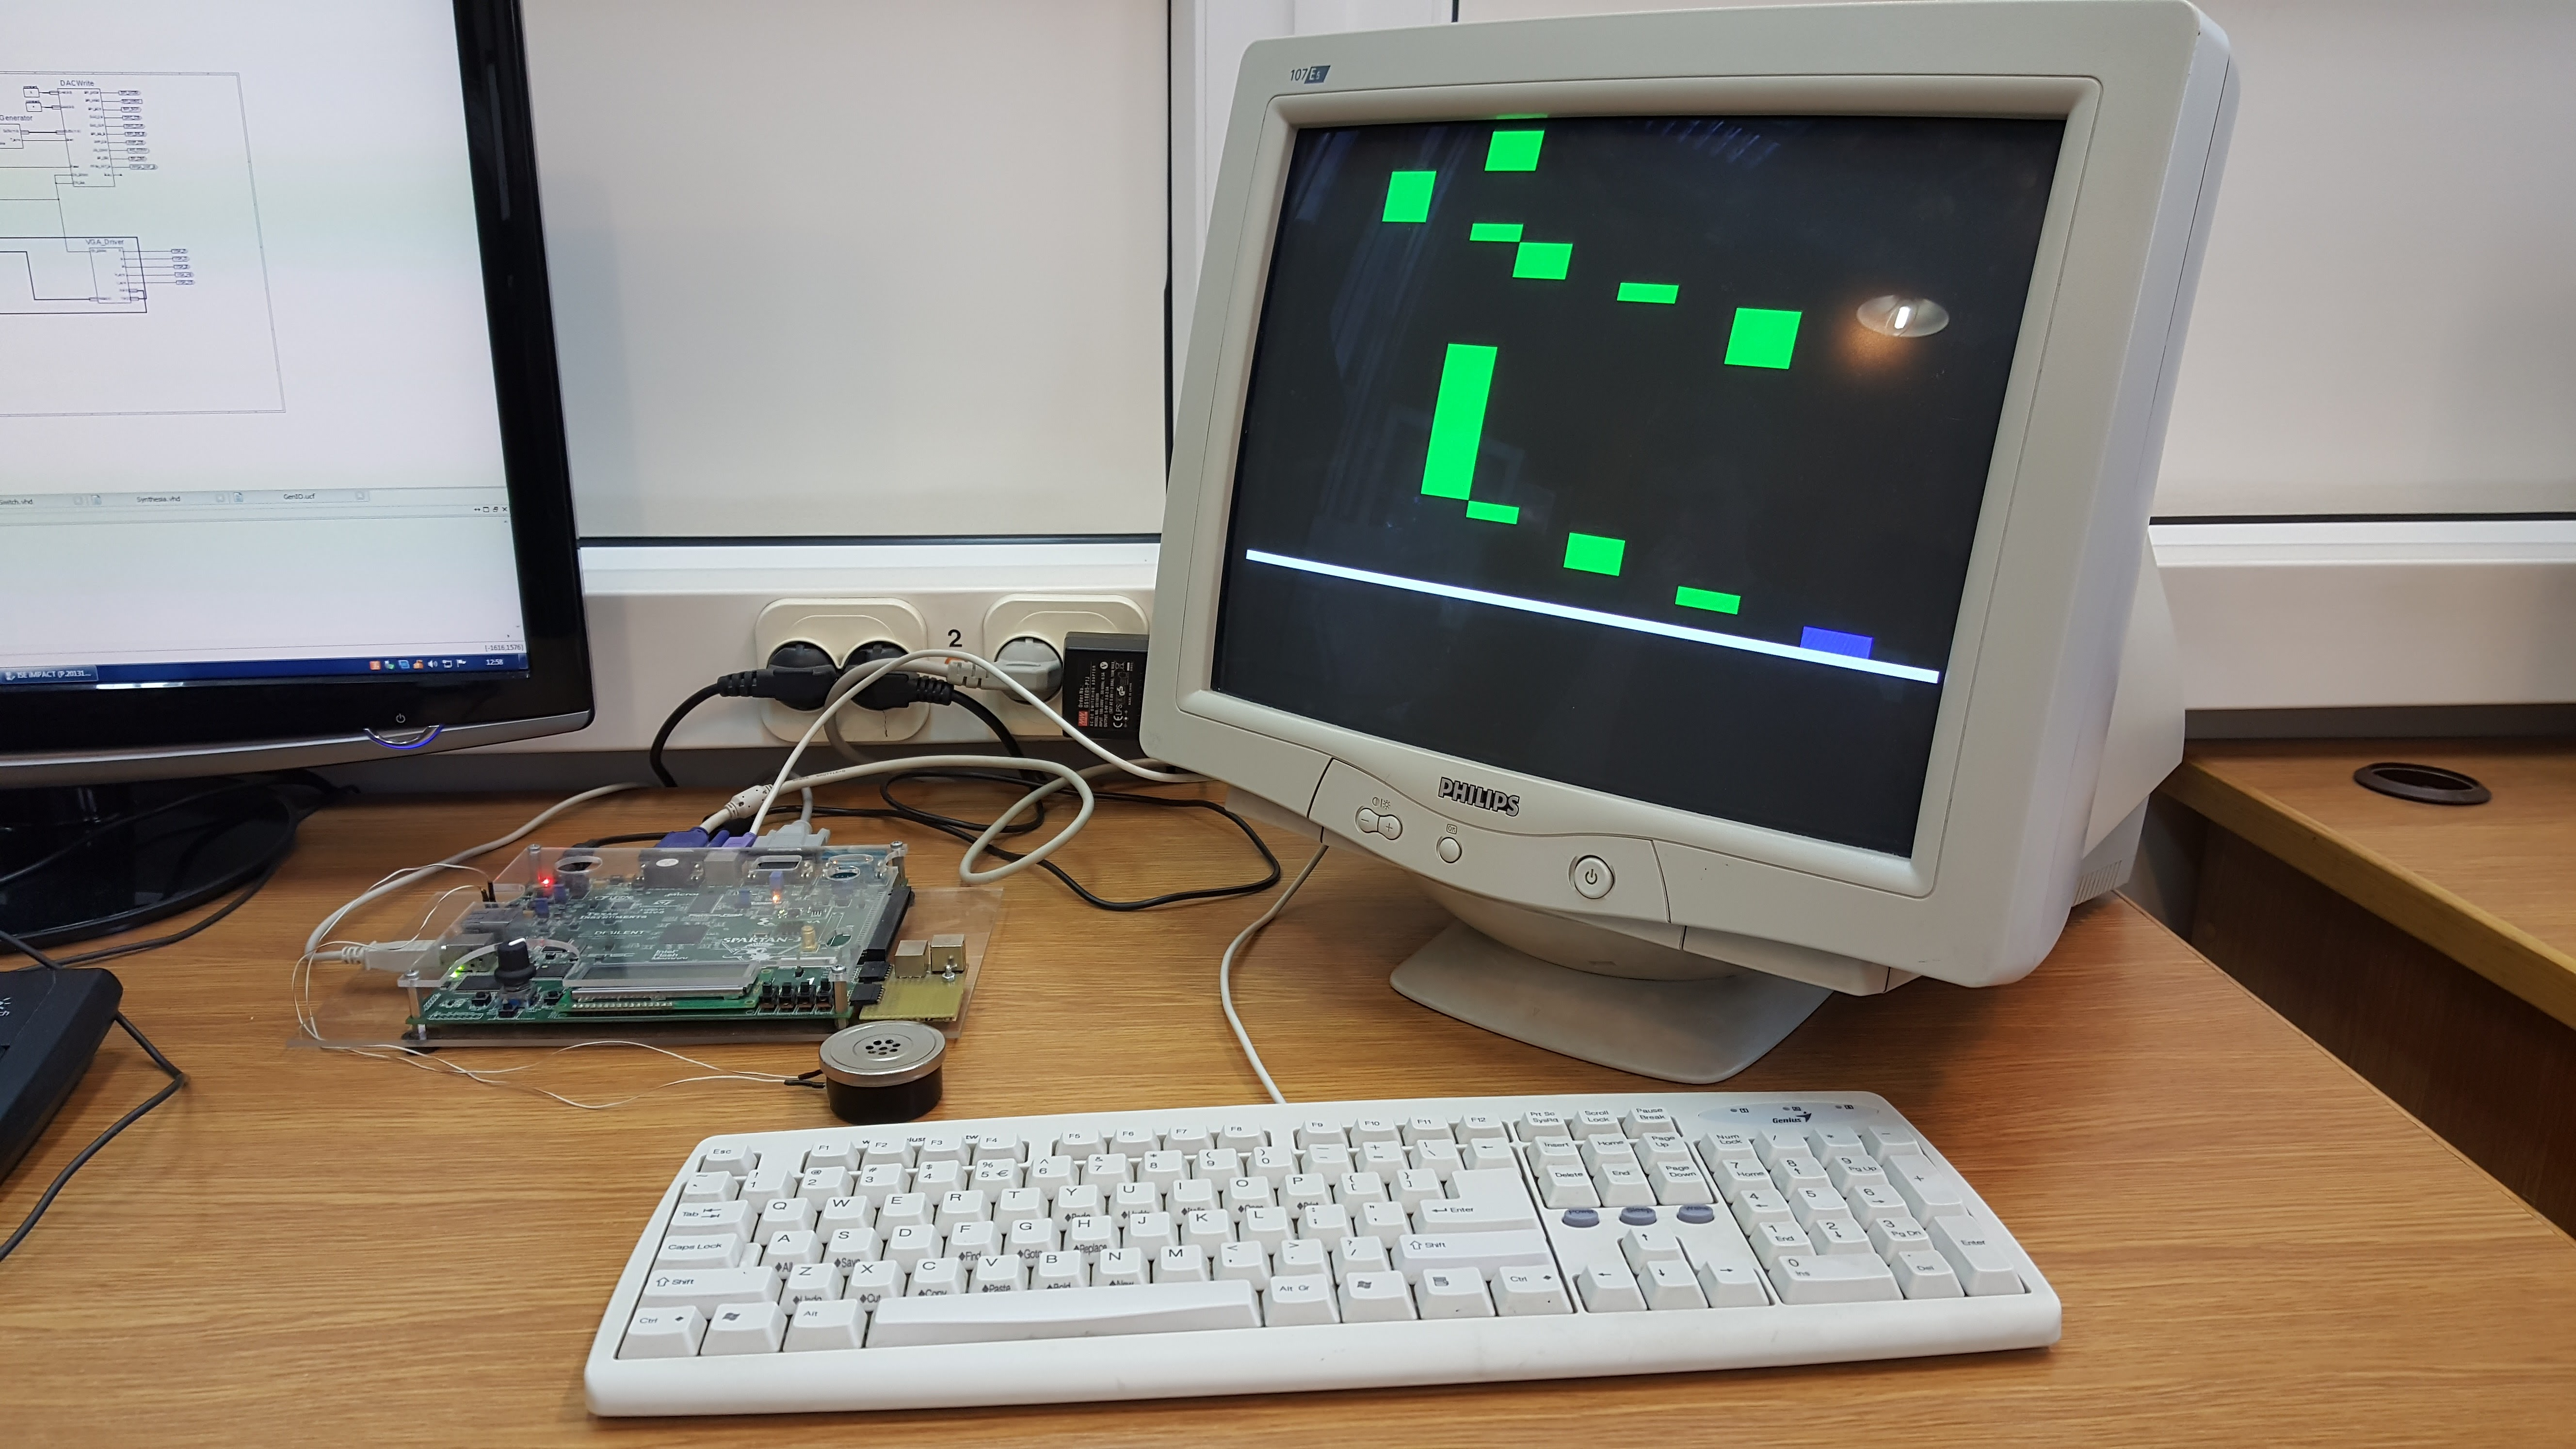
\includegraphics[width=1.0\textwidth]{zestaw_calosc.jpg}
				\caption{Zestaw - całość}
	\end{figure}	
		
	
\chapter{Podsumowanie}
	\section{Ocena krytyczna}
	Pierwsza wersja założeń projektowych nie została wykonana ze względu na ograniczenia czasowe oraz zbyt dużą złożoność problemu zaplanowanej początkowo gry. Jednak wykonanie projektu zgodnie z \\nowymi założeniami jest dobrym wstępem do stworzenia pierwotnie zaplanowanej gry. Wszystkie nowsze założenia udało się spełnić. Podstawowe funkcje takie jak wyświetlanie animacji i odgrywanie melodii zapisanej w pamięci urządzenia, tryb swobodnej gry i możliwość swobodnego przechodzenia między tymi trybami zostały przetestowane zarówno przy pomocy testów w środowisku ModelSim, jak również manualnie w sali laboratoryjnej.
\\\\ Podczas tworzenia projektu, szczególna uwaga została przywiązana do stworzenia systemu rozszerzalnego o nowe funkcje. Stworzony został system zapisu dźwięków o zadanej długości. Generowane dźwięki można zmieniać definiując ich częstotliwość, ale również możliwe jest łatwe dodawanie nowych dźwięków do już istniejących.
\\\\Pomimo tego, że nie udało się stworzyć gry, sama pozytywka odgrywająca melodię jednocześnie \\wyświetlając graficzną reprezentację melodii na ekranie wymagało dużego nakładu pracy i odpowiedniego podejścia do złączenia niezależnych elementów systemu w całość.
	\section{Kierunki dalszych prac}
	Pierwszym kierunkiem w którego stronę mógłby zmierzyć powyższy projekt jest stworzenie gry poprzez dodanie modułu zarządzającego relacją modułów Synthesia - Klawiatura. Projekt można również \\zmodyfikować poprzez zamianę klawiatury komputerowej na klawiaturę MIDI. \\\\Wartym rozważenia pomysłem jest również dołączenie głośnika stereo oraz dodanie możliwości zagrania więcej niż jednego dźwięku naraz, aby gra na syntezatorze była bardziej zbliżona do gry na prawdziwym instrumencie. Dobrym rozwiązaniem byłoby również dołączenie możliwości odczytu melodii z karty pamięci lub możliwości nagrania własnej melodii w celu późniejszego odtworzenia.\\\\W przypadku wyświetlacza, warto byłoby również rozważyć stworzenie menu systemu z możliwością edycji odpowiednich opcji lub ustawiania odpowiednich trybów pracy systemu.
	
\begin{thebibliography}{999}
		\bibitem{Spartan} 
		{\em http://www.xilinx.com/support/documentation/boards\_and\_kits/ug230.pdf}, \\
		dokumentacja układu Spartan-3E Starter Kit Board.
	
		\bibitem{Lesson 104 VGA Controller} 
		{\em https://www.youtube.com/watch?v=wzhDRIX2Ors}, \\
		film prezentujący zasady działania kontrolerów VGA.
		
		\bibitem{Numeric STD} 
		{\em http://staff.iiar.pwr.wroc.pl/antoni.sterna/ucsw/numeric\_std.pdf}, \\
		dokument opisujący konwersje typów przy użyciu biblioteki IEEE.numeric\_std.
		
			\bibitem{Scan Codes} 
		{\em http://www.computer-engineering.org/ps2keyboard/scancodes2.html}, \\
		tabela kodów interfejsu klawiatury PS/2.
		
	\end{thebibliography}	

% Compile twice to generate list of tables and figures properly
\begin{appendix}
	\listoffigures
\end{appendix}



\end{document}
